\documentclass[tikz,border=8pt]{standalone}
\begin{document}
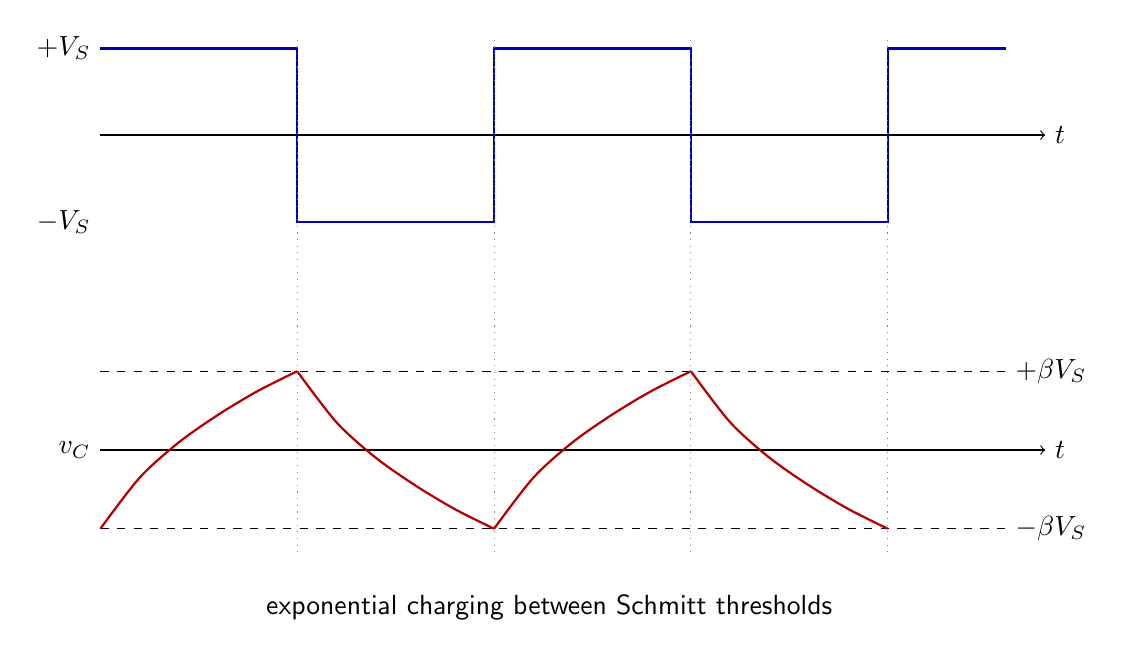
\begin{tikzpicture}[font=\sffamily,x=1cm,y=1cm]
\draw[->] (0,0)--(12,0) node[right]{$t$};
\draw[blue!70!black,thick] (0,1.1)--(2.5,1.1)--(2.5,-1.1)--(5,-1.1)--(5,1.1)--(7.5,1.1)--(7.5,-1.1)--(10,-1.1)--(10,1.1)--(11.5,1.1);
\node[left] at (0,1.1) {$+V_S$}; \node[left] at (0,-1.1) {$-V_S$};
\draw[->] (0,-4)--(12,-4) node[right]{$t$};
\draw[dashed] (0,-3)--(11.5,-3) node[right]{$+\beta V_S$};
\draw[dashed] (0,-5)--(11.5,-5) node[right]{$-\beta V_S$};
\draw[red!70!black,thick] plot[smooth] coordinates {(0,-5)(.5,-4.35)(1,-3.9)(1.5,-3.55)(2,-3.25)(2.5,-3)};
\draw[red!70!black,thick] plot[smooth] coordinates {(2.5,-3)(3,-3.65)(3.5,-4.1)(4,-4.45)(4.5,-4.75)(5,-5)};
\draw[red!70!black,thick] plot[smooth] coordinates {(5,-5)(5.5,-4.35)(6,-3.9)(6.5,-3.55)(7,-3.25)(7.5,-3)};
\draw[red!70!black,thick] plot[smooth] coordinates {(7.5,-3)(8,-3.65)(8.5,-4.1)(9,-4.45)(9.5,-4.75)(10,-5)};
\foreach \x in {2.5,5,7.5,10}{\draw[gray,dotted] (\x,-5.3)--(\x,1.25);}
\node[left] at (0,-4) {$v_C$};
\node at (5.7,-6) {exponential charging between Schmitt thresholds};
\end{tikzpicture}
\end{document}
